\section{Zielsetzung}
\label{sec:Ziel}
Das Ziel des Versuches ist die Verifikation der Fresnelschen Formeln durch Intensitätsmessungen eines an Silizium reflektierten Laserstrahls. Es soll ein experimenteller
Wert des Brechungsindizes von Silizium und des Brewsterwinkels bestimmt werden.

\section{Theorie}
\label{sec:Theorie}
Trifft Licht auf eine Grenzfläche zweier Medien, so wird in aller Allgemeinheit ein Teil des Lichtstrahls reflektiert und ein Teil transmittiert. Der reflektierte Teil
wird im selben Winkel zum Lot reflektiert, indem die einfallende Welle auf die Grenzfläche trifft. Der transmittierte Teil wird aufgrund der unterschiedlichen 
Ausbreitungsgeschwindigkeiten des Lichtes in den zwei Medien gebrochen und läuft anschließend in einem Winkel $\beta$ weiter. Das \textit{Snelliussche Brechungsgesetz}
\begin{equation}
    \label{eqn:Snellius}
    n_{1} \sin(\alpha)=n_{2} \sin(\beta)
\end{equation}
liefert einen Zusammenhang zwischen den Brechungsindizes $n_1$ und $n_2$ der beiden Medien und den jeweiligen Winkeln.
In diesem Versuch wird die Grenzfläche zwischen Luft und Silizium betrachtet, weshalb der Brechungsindex $n_1 = n_\text{Luft} \approx 1$ in den folgenden Rechnungen
verwendet wird.

Da Licht eine elektromagnetische Welle (\textit{e-m}-Welle) ist, wird die Ausbreitung von Licht durch die \textit{Maxwellschen Gleichungen} beschrieben. Die messbare Intensität 
einer Lichtquelle verhält sich proportional zur Amplitude des $\vec{E}$-Feld-Anteiles der \textit{e-m}-Welle, welcher aufgrund der hohen Frequenz nicht direkt gemessen werden 
kann. Dies bietet die Möglichkeit durch eine Intensitätsmessung auf die Amplitude des $\vec{E}$-Feldes eines Lichtstrahls zu schließen.

\subsection{Herleitung der Fresnelschen Formeln}
\label{subsec:T_Fresnel}
Die Strahlungsleistung einer \textit{e-m}-Welle wird durch den \textit{Poynting-Vekor} $\vec{S} = \vec{E} \times \vec{H}$ beschrieben. Durch den Zusammenhang der 
elektrostatischen- und magnetischen Felder über die Maxwell-Gleichungen ergibt sich der Betrag
\begin{equation}
    \label{eqn:Betrag_S}
    |\vec{S}| = c \varepsilon_0 \varepsilon \vec{E}^2
\end{equation}
des Poynting-Vektors. Dabei sind $\varepsilon_0$ und $\varepsilon$ die Permittivität des Vakuums, beziehungsweise die materialabhängige relative Permittivität und $c$ die 
Ausbreitungsgeschwindigkeit des Lichtes in einem Medium.    
Über eine Energiebetrachtung der Strahlenbündel kann mithilfe des Betrages des Poynting-Vektors die Gleichung
\begin{equation*}
    S_\text{e} \cos(\alpha) = S_\text{r} \cos(\alpha) + S_\text{t} \cos(\beta)
\end{equation*}
hergeleitet werden, wobei $S_i$ der Betrag des Poynting-Vektors der einfallenden (e), transmittierten (t) und reflektierten (r) Teilstrahlen ist.
Eine geometrische Veranschaulichung der Situation ist in \autoref{fig:Reflexion_Brechung} dargestellt.
\begin{figure}
    \centering
    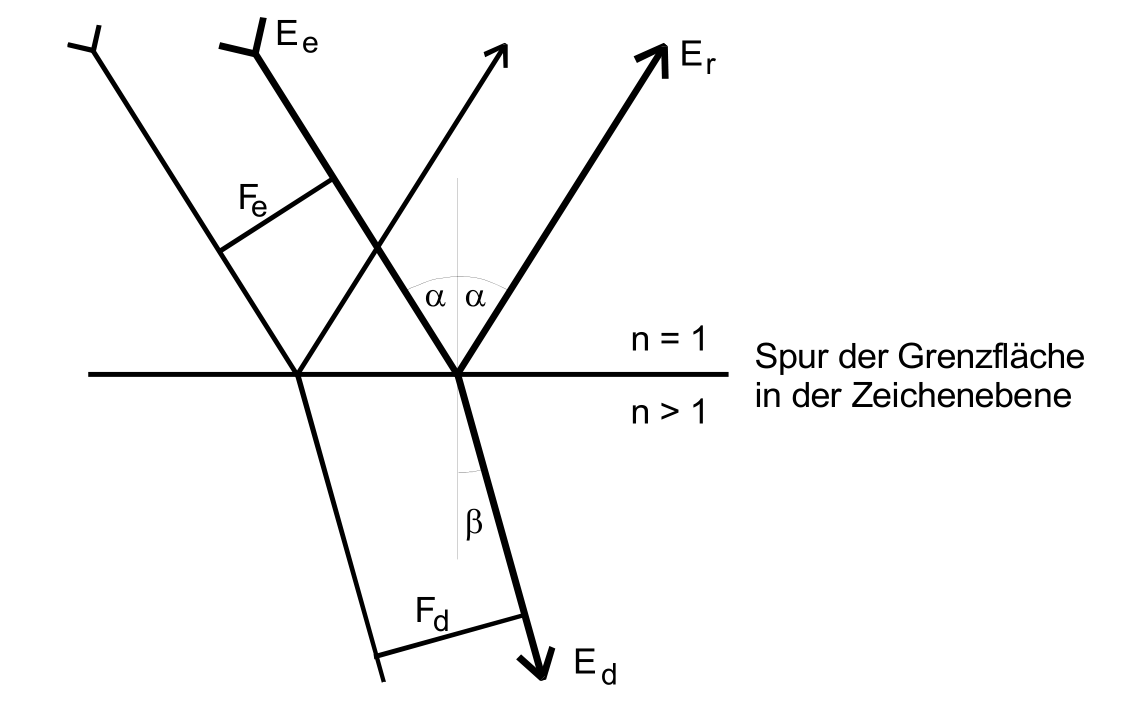
\includegraphics[width = .65\textwidth]{content/Reflexion_Brechung.png}
    \caption{Darstellung der Reflexion und Brechung einer einfallenden Welle an einer Grenzfläche \cite{v407}.}
    \label{fig:Reflexion_Brechung}
\end{figure}
Durch Einsetzen von \eqref{eqn:Betrag_S}, $n^2 = \varepsilon$ (für nicht ferromagnetische Stoffe) und $c^2 = \sfrac{1}{\varepsilon \varepsilon_0 \mu_0}$ folgt
\begin{equation*}
    \left(\vec{E}_\text{e}^2 - \vec{E}_\text{r}^2\right) \cos(\alpha) = n \vec{E}_\text{t}^2 \cos{\beta}.
\end{equation*}
Wenn der Feldvektor $\vec{E}_\text{e}$ der eintreffenden Welle in seine senkrecht- (s) und parallel- (p) zur Einfallsebene polarisierten Anteile 
\begin{equation*}
    \vec{E}_\text{e} = \vec{E}_\text{e,s} + \vec{E}_\text{e,p}
\end{equation*}
unterteilt wird, lassen sich mit den Stetigekeitsbedingungen
\begin{align*}
    \vec{E}_\text{e,s} + \vec{E}_\text{r,s} &= \vec{E}_\text{t,s} \\
    \left(\vec{E}_\text{e,p} - \vec{E}_\text{r,p}\right) \cos(\alpha) &= \vec{E}_\text{t,p} \cos(\beta)
\end{align*}
an der Grenzfläche
die Fresnelschen Formeln herleiten. Dazu werden die p- und s- polarisierten Anteile einzeln betrachtet, $\vec{E}_\text{t}$ durch die 
Stetigkeitsbedingungen eliminiert und der Brechugnswinkel $\beta$ mithilfe des Snelliusschen Brechungsgesetz \eqref{eqn:Snellius} ersetzt. 
Für die reflektierte Amplitude des senkrecht polarisierten Anteils folgt
\begin{equation}
    \label{eqn:Fresnel_senkrecht}
    \vec{E}_\text{r,s} = -\vec{E}_\text{e,s} \cdot \frac{\left(\sqrt{n^2 - \sin^2(\alpha)} -\cos(\alpha)\right)^2}{n^2 - 1}
    %&= \vec{E}_\text{e,s} \frac{\cos(\alpha)- \sqrt{n^2 - \sin^2(\alpha)}}{\cos(\alpha) + \sqrt{n^2 - \sin^2(\alpha)}}.
\end{equation}
Der parallel polarisierte Anteil kann durch
\begin{equation}
    \label{eqn:Fresnel_parallel}
    \vec{E}_\text{r,p} = \vec{E}_\text{e,p} \cdot \frac{n^2 \cos(\alpha) - \sqrt{n^2 - \sin^2(\alpha)}}{n^2 \cos(\alpha) + \sqrt{n^2 - \sin^2(\alpha)}}
\end{equation}
berechnet werden.

\subsection{Der Brewster-Winkel}
\label{subsec:T_Brewster}
Die Fresenelsche Formel für den parallel polarisierten Anteil lässt sich auch als 
\begin{equation*}
    \vec{E}_\text{r,p} = \vec{E}_\text{e,p} \cdot \frac{\tan(\alpha - \beta)}{\tan(\alpha + \beta)}
\end{equation*}
schreiben und verschwindet somit für $\alpha_\text{B} + \beta_\text{B} = \sfrac{\pi}{2}$ aufgrund der Divergenz des Tangens. Daraus folgt mit dem Snelliusschen Brechungsgesetz und $n_1 = 1$
\begin{align}
    \sin(\alpha_\text{B}) &= n \cdot \sin(\sfrac{\pi}{2} - \alpha_\text{B}) = n \cdot \cos(\alpha_\text{B}) \nonumber \\
    \Leftrightarrow n &= tan(\alpha_B)
    \label{eqn:Brewster}
\end{align}
für den Brechungsindex $n$ des betrachteten Materials (hier Silizium).
Ein Lichtstrahl, der unter dem Brewster-Winkel $\alpha_\text{B}$ einfällt wird also vollständig transmittiert.
